\documentclass{mimosis}

\usepackage{metalogo}
\usepackage{xargs}                      % Use more than one optional parameter in a new commands
\usepackage{indentfirst}
%
\usepackage[colorinlistoftodos,prependcaption,textsize=tiny]{todonotes}
\newcommandx{\unsure}[2][1=]{\todo[linecolor=red,backgroundcolor=red!25,bordercolor=red,#1]{#2}}
\newcommandx{\change}[2][1=]{\todo[linecolor=blue,backgroundcolor=blue!25,bordercolor=blue,#1]{#2}}

\newcommandx{\info}[2][1=]{\todo[linecolor=OliveGreen,backgroundcolor=OliveGreen!25,bordercolor=OliveGreen,#1]{#2}}
\newcommandx{\improvement}[2][1=]{\todo[linecolor=Plum,backgroundcolor=Plum!25,bordercolor=Plum,#1]{#2}}
\newcommandx{\thiswillnotshow}[2][1=]{\todo[disable,#2]{#1}}
%

\usepackage{float}
\usepackage{geometry}
\usepackage{babel}
\usepackage{svg}
\graphicspath{ {./img/} }

\newcommand{\alphabet}{%
  abcdefghijklmnopqrstuvwxyz%
}
\newlength{\textW}
\setlength{\textW}{\widthof{\alphabet}* \real{2.5}}
\geometry{textwidth=\textW,}
\newcommand{\myref}[2]{\hyperref[#2]{#1~\ref*{#2}}}
%%%%%%%%%%%%%%%%%%%%%%%%%%%%%%%%%%%%%%%%%%%%%%%%%%%%%%%%%%%%%%%%%%%%%%%%
% Some of my favourite personal adjustments
%%%%%%%%%%%%%%%%%%%%%%%%%%%%%%%%%%%%%%%%%%%%%%%%%%%%%%%%%%%%%%%%%%%%%%%%
%
% These are the adjustments that I consider necessary for typesetting
% a nice thesis. However, they are *not* included in the template, as
% I do not want to force you to use them.

% This ensures that I am able to typeset bold font in table while still aligning the numbers
% correctly.
\usepackage{etoolbox}
\usepackage{listings}
\lstset{
  basicstyle=\ttfamily,
  columns=fullflexible,
  frame=single,
  keywordstyle=\color{red},
  breaklines=true,
  postbreak=\mbox{\textcolor{red}{$\hookrightarrow$}\space},
}


\usepackage{dirtree}

\usepackage[binary-units=true]{siunitx}
\DeclareSIUnit\px{px}

\sisetup{%
  detect-all           = true,
  detect-family        = true,
  detect-mode          = true,
  detect-shape         = true,
  detect-weight        = true,
  detect-inline-weight = math,
}

%%%%%%%%%%%%%%%%%%%%%%%%%%%%%%%%%%%%%%%%%%%%%%%%%%%%%%%%%%%%%%%%%%%%%%%%
% Hyperlinks & bookmarks
%%%%%%%%%%%%%%%%%%%%%%%%%%%%%%%%%%%%%%%%%%%%%%%%%%%%%%%%%%%%%%%%%%%%%%%%

\usepackage[%
  colorlinks = true,
  citecolor  = OliveGreen,
  linkcolor  = Mahogany,
  urlcolor   = RoyalBlue,
  unicode,
  ]{hyperref}


\newcommand{\smallquote}[1]{
    \begin{center}
        \begin{minipage}{0.5\textwidth}
            \begin{small}
                #1
            \end{small}
        \end{minipage}
        \vspace{0.5cm}
    \end{center}
}

\usepackage{bookmark}

\usepackage[all]{nowidow}

%%%%%%%%%%%%%%%%%%%%%%%%%%%%%%%%%%%%%%%%%%%%%%%%%%%%%%%%%%%%%%%%%%%%%%%%
% Bibliography
%%%%%%%%%%%%%%%%%%%%%%%%%%%%%%%%%%%%%%%%%%%%%%%%%%%%%%%%%%%%%%%%%%%%%%%%
%
% I like the bibliography to be extremely plain, showing only a numeric
% identifier and citing everything in simple brackets. The first names,
% if present, will be initialized. DOIs and URLs will be preserved.

\usepackage[%
  autocite     = plain,
  backend      = biber,
  doi          = true,
  url          = true,
  giveninits   = true,
  hyperref     = true,
  maxbibnames  = 99,
  maxcitenames = 99,
  sortcites    = true,
  style        = iso-numeric,
  ]{biblatex}

%%%%%%%%%%%%%%%%%%%%%%%%%%%%%%%%%%%%%%%%%%%%%%%%%%%%%%%%%%%%%%%%%%%%%%%%
% Some adjustments to make the bibliography more clean
%%%%%%%%%%%%%%%%%%%%%%%%%%%%%%%%%%%%%%%%%%%%%%%%%%%%%%%%%%%%%%%%%%%%%%%%
%
% The subsequent commands do the following:
%  - Removing the month field from the bibliography
%  - Fixing the Oxford commma
%  - Suppress the "in" for journal articles
%  - Remove the parentheses of the year in an article
%  - Delimit volume and issue of an article by a colon ":" instead of
%    a dot ""
%  - Use commas to separate the location of publishers from their name
%  - Remove the abbreviation for technical reports
%  - Display the label of bibliographic entries without brackets in the
%    bibliography
%  - Ensure that DOIs are followed by a non-breakable space
%  - Use hair spaces between initials of authors
%  - Make the font size of citations smaller
%  - Fixing ordinal numbers (1st, 2nd, 3rd, and so) on by using
%    superscripts

% Remove the month field from the bibliography. It does not serve a good
% purpose, I guess. And often, it cannot be used because the journals
% have some crazy issue policies.
\AtEveryBibitem{\clearfield{month}}
\AtEveryCitekey{\clearfield{month}}

% Fixing the Oxford comma. Not sure whether this is the proper solution.
% More information is available under [1] and [2].
%
% [1] http://tex.stackexchange.com/questions/97712/biblatex-apa-style-is-missing-a-comma-in-the-references-why
% [2] http://tex.stackexchange.com/questions/44048/use-et-al-in-biblatex-custom-style
%
\AtBeginBibliography{%
  \renewcommand*{\finalnamedelim}{%
    \ifthenelse{\value{listcount} > 2}{%
      \addcomma
      \addspace
      \bibstring{and}%
    }{%
      \addspace
      \bibstring{and}%
    }
  }
}

% Suppress "in" for journal articles. This is unnecessary in my opinion
% because the journal title is typeset in italics anyway.
\renewbibmacro{in:}{%
  \ifentrytype{article}
  {%
  }%
  % else
  {%
    \printtext{\bibstring{in}\intitlepunct}%
  }%
}

% Remove the parentheses for the year in an article. This removes a lot
% of undesired parentheses in the bibliography, thereby improving the
% readability. Moreover, it makes the look of the bibliography more
% consistent.
\renewbibmacro*{issue+date}{%
  \setunit{\addcomma\space}
    \iffieldundef{issue}
      {\usebibmacro{date}}
      {\printfield{issue}%
       \setunit*{\addspace}%
       \usebibmacro{date}}%
  \newunit}

% Delimit the volume and the number of an article by a colon instead of
% by a dot, which I consider to be more readable.
\renewbibmacro*{volume+number+eid}{%
  \printfield{volume}%
  \setunit*{\addcolon}%
  \printfield{number}%
  \setunit{\addcomma\space}%
  \printfield{eid}%
}

% Do not use a colon for the publisher location. Instead, connect
% publisher, location, and date via commas.
\renewbibmacro*{publisher+location+date}{%
  \printlist{publisher}%
  \setunit*{\addcomma\space}%
  \printlist{location}%
  \setunit*{\addcomma\space}%
  \usebibmacro{date}%
  \newunit%
}

% Ditto for other entry types.
\renewbibmacro*{organization+location+date}{%
  \printlist{location}%
  \setunit*{\addcomma\space}%
  \printlist{organization}%
  \setunit*{\addcomma\space}%
  \usebibmacro{date}%
  \newunit%
}

% Display the label of a bibliographic entry in bare style, without any
% brackets. I like this more than the default.
%
% Note that this is *really* the proper and official way of doing this.
\DeclareFieldFormat{labelnumberwidth}{#1\adddot}

% Ensure that DOIs are followed by a non-breakable space.
\DeclareFieldFormat{doi}{%
  \mkbibacro{DOI}\addcolon\addnbspace
    \ifhyperref
      {\href{http://dx.doi.org/#1}{\nolinkurl{#1}}}
      %
      {\nolinkurl{#1}}
}

\DefineBibliographyStrings{english}{
  online = {online}
}

\DefineBibliographyStrings{english}{
  urlalso = {Available from}
}


% Use proper hair spaces between initials as suggested by Bringhurst and
% others.
\renewcommand*\bibinitdelim {\addnbthinspace}
\renewcommand*\bibnamedelima{\addnbthinspace}
\renewcommand*\bibnamedelimb{\addnbthinspace}
\renewcommand*\bibnamedelimi{\addnbthinspace}

% Make the font size of citations smaller. Depending on your selected
% font, you might not need this.
\renewcommand*{\citesetup}{%
  \biburlsetup
  \small
}

\DeclareLanguageMapping{english}{english-mimosis}


\addbibresource{Thesis.bib}

%%%%%%%%%%%%%%%%%%%%%%%%%%%%%%%%%%%%%%%%%%%%%%%%%%%%%%%%%%%%%%%%%%%%%%%%
% Fonts
%%%%%%%%%%%%%%%%%%%%%%%%%%%%%%%%%%%%%%%%%%%%%%%%%%%%%%%%%%%%%%%%%%%%%%%%

\ifxetexorluatex
  \setmainfont{Minion Pro}
\else
  \usepackage[lf]{ebgaramond}
  \usepackage[oldstyle,scale=0.7]{sourcecodepro}
  \singlespacing
\fi

\renewcommand{\th}{\textsuperscript{\textup{th}}\xspace}


\makeindex
\makeglossaries

%%%%%%%%%%%%%%%%%%%%%%%%%%%%%%%%%%%%%%%%%%%%%%%%%%%%%%%%%%%%%%%%%%%%%%%%
% Incipit
%%%%%%%%%%%%%%%%%%%%%%%%%%%%%%%%%%%%%%%%%%%%%%%%%%%%%%%%%%%%%%%%%%%%%%%%

\title{Trusted Platform Modules: visualization of the performance data}
\author{Tomáš Jaroš}

% This ensures that the subsequent sections are being included as root
% items in the bookmark structure of your PDF reader.
\begin{document}
\frontmatter
    \begin{titlepage}
  \vspace*{2cm}
  \makeatletter
  \begin{center}
      \begin{LARGE}
          \textsc{Masaryk University}
      \end{LARGE}\\[0.01cm]
      \begin{Large}
          \textsc{Faculty of Informatics\\}
      \end{Large}
      \vspace*{1cm}
      
\includegraphics[width=40mm]{fithesis-fi.pdf}\\
      \vspace*{3cm}
    \begin{Huge}
      \@title
    \end{Huge}\\[1.5cm]
    %
    \begin{Large}
        \textsc{Bachelor's Thesis}
    \end{Large}\\[1.5cm]
    %
    \begin{LARGE}
        \@author
    \end{LARGE}
    %
    \vfill
  \end{center}
  \begin{flushright}
      \begin{large}
        May 2022
      \end{large}
  \end{flushright}
  \makeatother
\end{titlepage}

\newpage
\null
\thispagestyle{empty}
\newpage


    %\chapter*{Declaration}

\noindent
Hereby I declare, that this thesis is my original work, which I
have worked out on my own. All sources, references and literature used or
excerpted during elaboration of this work are properly cited and listed in
complete reference to the due source.

\vspace{1cm}
\begin{flushright}
    Tomáš Jaroš
\end{flushright}
\vfill
\textbf{Advisor:} doc. RNDr. Petr Švenda, Ph.D.

    %\chapter*{Acknowledgements}
\noindent
I want to express my utmost gratitude to my advisor, doc. Petr Švenda, for his professional guidance, patience, and helpful advice he provided me during the preparation of this thesis. I would also like to thank my family for their immense support and encouragement throughout my studies.
    %\chapter*{Abstract}
\noindent


\section*{Keywords}
\noindent
% TODO

    \tableofcontents
    \listoffigures
    \glsaddall
    %\printglossary[type=\acronymtype]
    \chapter{Introduction}
The Trusted Platform Module is a device designed to enhance the security of computing platforms. Many different vendors produce these devices while adhering to the standardized specifications, which define both the mandatory and the optional components. This results in devices having the required functionality in common, but the optional functionality is left to the device architects to include. Thus the produced devices may vary in functionality and performance because the implementation details vary across different vendors.

The objective of this thesis is to implement a tool for the visualization of data collected from Trusted Platform Modules. The resulting tool should be able to create visualizations for several datasets which report on supported functionality, performance characteristics, and cryptographic properties. The visualizations should also be compatible with datasets that report on similar information collected from different secure devices, the JavaCard smart cards.

The first chapter provides an overview of Trusted Platform Module technology. The second chapter analyses the current state of an existing solution for visualization and describes design decisions behind the tool created as the objective of this thesis. The final chapter  presents the outcome of this thesis, a tool called \texttt{AlgTest pyProcess}.




\mainmatter
  \chapter{State of the Art}

\section{Trusted Platform Module}
The Trusted Platform Module is a system component used as a cryptographic co-processor. It was developed by and standardized by the Trusted Computing Group (TCG) consortium with the purpose of laying a foundation on which secure systems could be further created and developed. 

\subsection{History}
The first broadly used specification was TPM 1.1b, released in 2003. TPMs released under this specification already provided some essential functions found in modern TPMs consisting of key generation of RSA key pairs, storage, secure authorisation, and device-health attestation. For the sake of assuring privacy, the
use of anonymous identity keys based on certificates was introduced. In order to take advantage of such
functionality, these certificates needed to be provided with the TPM, and any generation of such keys was available only after owner authorisation. To be able to anonymously prove the origin of the keys generated
by TPM, a \texttt{privacy certification authority} was created. The integrity of measurements collected during systems boot sequence is provided by Platform Configuration Registers (PCRs). Both PCRs and identity keys might have been used to prove the health of the system's boot sequence~\cite{arthur2015practical}.


The hardware specification was not standardized in TPM 1.1b. This caused various incompatibilities. The TPMs across different vendors provided differing interfaces, which required different drivers. Pin-outs on the chips were not prescribed by any standard. Additionally, there were no countermeasures against dictionary attacks~\cite{arthur2015practical}.
% Should i also mention DAA ?

While being in development from 2005 to 2009, the TPM 1.2 specification went through numerous releases. Regarding the need to store shipped certificates for TPM's endorsement keys on a hard disk, about 2KB of non-volatile RAM was added. A new design needed to be made to support key migration between different TPMs because the old design of key migration would in TPM 1.12 require users to have TPM owner authorization. The new idea made users able to create migratable keys and then relied on a designated third party that could exclusively migrate such keys. Said keys could also be certified. Thus, they were called Certified Migratable keys. Additionally, an internal timer able to synchronize with the external one was added in 1.12, which has its use when signing data due to timestamps. Version 1.12 required API to provide backward compatibility for 1.1b. This increased the complexity of the new specification. The TPM 1.12 became widely used in x86 personal computers starting 2005 and later in 2008 also in servers~\cite{arthur2015practical}.

One of the factors that contributed to the need for yet another specification after TPM 1.12 was that in 2005, some substantial collision attacks were found against the SHA-1 hash function. Analysis regarding the use of SHA-1 in TPM revealed the attacks not being applicable~\cite{tcg_tpm1.12_sha-1_uses}. Due to the extensive use of SHA-1 in TPM 1.12, the new specification had to permit any hashing algorithm without the need to make any changes to the specification. A so-called \texttt{digest agility}. Another problem was the lack of a symmetric algorithm required in the TPM specification. The use of RSA for encryption of serialized data was impractical because RSA operations are slow. Neither would help support bigger-sized RSA keys because that would cause a higher chip cost, incompatibility issues, and lower performance. That's why it was decided that the following specification would adopt support for symmetric encryption, which is faster and more suitable for encryption of large byte streams. Having this many problems, an overhaul of the specification would be convenient. And the architects of TPM 2.0 took advantage of the situatio~\cite{arthur2015practical}.


\subsection{Features}


\section{Performance analysis}
\subsection{tpm2-algtest}
The \texttt{tpm2-algtest}\footnote{https://github.com/crocs-muni/tpm2-algtest} is a tool for automatic gathering of information about the TPM2 devices \cite{Struk2019thesis}. The tool uses libraries implementing Trusted Computing Group's TPM2 Software Stack\footnote{https://github.com/tpm2-software/tpm2-tss} which allows for simplification of development when programming applications supposed to interact with the TPM. The tool tests for support of specific commands and supporting routines, values of structures defined in the TPM 2.0 specification \cite{tcg_p3_commands, tcg_p4_supproutines, tcg_p2_structures}. Supported cryptographic algorithms are also subject to performance analysis where the time to execute such an algorithm is repeatedly measured and recorded. Additionally, the tool uses the TPM to generate key pairs for RSA and ECC-based algorithms so that they can be further analyzed by various means.
be dodo
  
  \chapter{Analysis and design}
One of the objectives of this work was the creation of a tool for processing and visualization of results from TPM devices. Such a tool already exists, and it is called \texttt{JCAlgTest process}. However, the tool's current design makes it difficult to extend it. Extensive refactoring could help in gaining more extensibility. Nevertheless, a complete rework proved more effective in this case.

This chapter describes the original tool for generating visualizations and discusses its problems. Then solutions to those problems are proposed, and it is described how they have been used in the reimplementation.

\section{JCAlgTest}\label{sec:jcalgtest}
The \texttt{JCAlgTest}\footnote{\url{https://github.com/crocs-muni/JCAlgTest}} is a suite of tools used for automated analysis of cryptographic smartcards, specifically those running the JavaCard platform. It takes advantage of the officially available JavaCard API to test for support of specific algorithms, measures their performance characteristics, and collects general information about the tested smart card. The suite consists of three modules:
\begin{itemize}
  \item
        \texttt{JCAlgTestJavaCard} is a JavaCard applet that needs to be uploaded onto the tested smart card. According to instructions from \texttt{JCAlgTestClient} application to execute code for specified operation. Firstly it tries to instantiate a particular object belonging to the operation. If it succeeds, that means that the operation is supported, and in the case of performance testing, it can proceed further with the execution. If the instantiation was unsuccessful, a specific exception is thrown, which usually means that the operation is not supported.
  \item
        \texttt{JCAlgTestClient} is a host application which is responsible for communication with \texttt{JCAlgTestJavaCard} applet via APDU commands and responses. The information about the algorithm execution time is measured and recorded. The JavaCard platform does not support any time measurement methods. The execution time measurement during the performance testing is estimated externally due to the limitations of the JavaCard platform, which does not support any time measurement methods. 
  \item
        \texttt{JCAlgTestProcess} is an application that is used for the visualization of JavaCard and TPM results. Results in the form of CSV files are processed into various kinds of visualizations and tabular data. As the state of the tool is deemed obsolete, its reimplementation was needed and was performed as one of the goals of this thesis. The reasons behind the reimplementation and the new design are discussed in the following sections.
\end{itemize}

\section{JCAlgTest process}
The \texttt{JCAlgTest process} is an application used for tabular and chart visualisations of JavaCard smart card and TPM 2.0 run time data created by \texttt{JCAlgTest} and \texttt{tpm2-algtest} tools respectively. 

This section will describe the application's current state and its problems.
\subsection{Current state}
%\todo{Add diagram visualising basic parts of the old app}

The application is written in Java programming language. It is designed mainly as a command-line tool for generating HTML visualizations for JavaCard smart card run time data. Still, it also contains means of visualizing TPM 2.0 run time data. The project's website shows JavaCard smart card visualizations \cite{jcalgtestWeb}. Each type of visualization is performed by building an HTML file and either by embedding JavaScript calls to visualization functions contained in  \texttt{D3.js library} or \texttt{Google Charts API} or by creating a basic HTML table with added CSS styling and usability improvements such as sorting or filtering of entries using JavaScript. 

An \texttt{Apache Ant} command-line tool is used to build the application. It uses XML files to describe the build processes such as compiling, running, or testing. It is also supported by many programming IDEs, most notably Netbeans IDE or IntelliJ IDEA.

The \texttt{JCAlgTest process} provides a command-line API. The users can specify the input, output directory, and the type of visualization they want to generate.

\subsection{Problems}\label{subsec:design-problems}
The whole \texttt{JCAlgTest} suite was developed over several years by various people. An initial version of \texttt{JCAlgTest Process} along with the rest of \texttt{JCAlgTest} suite was created by doc. Petr Švenda, my supervisor. Following that, Rudolf Kvašňovský further developed the \texttt{JCAlgTest process} tool as a part of his bachelor's thesis~\cite{Kvasnovsky2016thesis}. From there on, several more minor updates from various people were performed. The application serves its intended purpose well, however, any extensions to it require lots of code analysis and patience so that nothing breaks and no new issues arise.

One of the problems of the application is the lack of object representation of device profiles. The data is primarily stored in simple Java array lists or maps. That is why a relatively simple task of extending functionality may prove to be very difficult. 

Another problem is the amount of hard-coded HTML tags into strings. One unintentional mistake of deleted angle bracket may corrupt the whole HTML output. To change, for instance, something in the metadata of each generated HTML, it is needed to manually change the string, which creates the body part of the HTML document. 

\section{Improvements}
In this section, the improvements for the \texttt{JCAlgTest process} tool will be discussed along with how they have been applied to its reimplementation.

\subsection{Object design}
As mentioned in \myref{Section}{subsec:design-problems}, the object design of the tool needed some improvements. The new design should provide classes mapping the information contained in input files. They will be referred to as device profiles. The device stands for either TPM 2.0 or JavaCard smart card. The data is in the form of CSV files. However, the format of some files does not conform to any specific implementation for CSV format, as there is no header for the data, and the count of delimiters is variable on each line. This effectively results in the need to parse files using custom-made parser procedures instead of relying on library functions.

\subsubsection{Device profile types}\label{sec:device-profiles}
There are three main types of device profiles:
\begin{enumerate}
    \item \textbf{Support} In the case of TPM devices, it contains information about the support of specific algorithms, commands, or structures defined in the TPM 2.0 specification. However, in the case of JavaCard smart cards, the information is about supported cryptographic algorithms defined in JavaCard API. Along with this information, it also contains basic information about the devices. This information ranges from vendor information to memory limits.
    
    \item \textbf{Performance} Contain run time benchmarks for cryptographic algorithms. Similarly, as in the previous case, the tested algorithms, commands, or structures originate from either TPM 2.0 specification for TPMs, or JavaCard API in the case of JavaCard smart cards. In the case of JavaCard smart cards, the performance results are divided into fixed and variable results. Variable-length performance results measure data length dependant performance, whereas fixed-length performance results measure it with static data length depending on a particular algorithm.
    
    \item \textbf{Cryptographic Properties} They contain information about the execution time duration for cryptographic algorithms supported by the TPM, additionally, they record the key pairs generated using RSA or ECC algorithms for analysis. The information is split into multiple data sets, and each data set contains only specific information about the tested TPM. The TPM is mentioned specifically because cryptographic properties in this form are recorded only for TPM devices.
\end{enumerate}

In the implementation, the object design of these profiles is very straightforward. The classes were modeled according to the information contained in the CSV files. Their objective is only to store the data so that it can be later manipulated. That is why there was no need for any complex abstractions in design. However, even such basic improvement by creating a class representation makes it easier to work with the data and the resulting code more readable compared to using array lists and indexes.

The profile classes are very similar. They all have to store specific results and other information inherited from their abstract base class. The measurement results are stored in dictionaries where we associate the identification of a result with its object or a list of these objects for easier checking if a specific result was measured.

The only exception to this system is the representation of profiles of cryptographic properties. These do not have a designed object form, but most of them are in the form of well-formed CSV files, so they can be manipulated using library functions.


\subsection{Building outputs}
Another problem to resolve was to find a way to build HTML outputs in a way where a small mistake does not result in a corrupted file and hours of debugging. One solution is a templating engine where we prepare a special file very similar to pure HTML with the exception of the special syntax that takes care of populating the template with data. This is the way more often used in modern front-end frameworks such as React or Vue. But templating may not always be the best idea, because it steepens the learning curve for understanding the code. That is because everyone needs to understand the new syntax used in the templates. The solution used in the reimplementation was the use of a library called \texttt{dominate} which makes us able to create HTML documents and fragments using pure Python language. Additionally, it was used in another project which also works with JavaCards called \texttt{scrutiny}, which was created as a part of a master's thesis by Imrich Nagy~\cite{Nagy2019thesis}. The reimplementation also uses some code from this project in case future extensions want to integrate some functionality from \texttt{scrutiny} into it.

%\subsection{Library approach}
%Another improvement worth mentioning is that the tool is divided into modules that provide separate  features such as parsing profiles or visualization. The classes used in the tool can be called from other environments supporting Python programming language by importing them. Examples of such environments are Jupyter\footnote{\url{https://jupyter.org}} based notebooks. An illustration of the usage of such a notebook is a part of the results of this thesis.

  \chapter{AlgTest pyProcess tool}
This chapter describes the development details behind the tool called \texttt{AlgTest pyProcess}, the creation of which was the main goal of this thesis. Its development began as a reimplementation of a tool called \texttt{JCAlgTest Process}. The reasons behind the reimplementation are mentioned in the previous chapter.

The \texttt{AlgTest pyProcess} tool is responsible for the following tasks:
\begin{itemize}
    \item Processing the device profiles generated by automatic testing tools targeted at Trusted Platform Modules and JavaCard smart cards,
    \item Generation of various outputs from these datasets which are primarily tabular and graphical visualizations.
\end{itemize}
\begin{figure}[h]
    \centering
    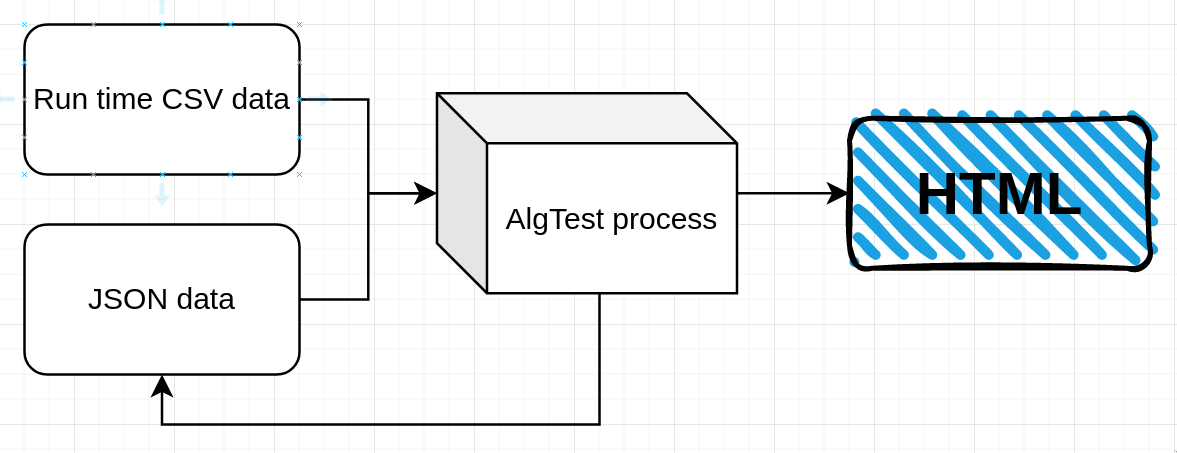
\includegraphics[width=\textwidth]{img/scheme.png}
    \caption{Scheme of AlgTest pyProcess application}
    \label{fig:algtest-process-scheme}
\end{figure}


\section{Parsing}
The \texttt{AlgTest pyProcess} tool is working with datasets that were generated and collected over the years in parallel with the development of the testing tools which generate these datasets. The outputs of these testing tools have been changing over the years too, that is why the testing form of output format for tested devices may differ depending on the version of the testing tool.

There is no prescribed schema for the datasets, but they generally look very similar\footnote{Examples of CSV device profiles are shown in Appendix}. That is why it is convenient to design suitable means of accessing the data contained in them. Such means are provided by mapping these profiles onto class representation. But the first step in order to accomplish that is the parsing of the CSV files which represent the device profiles. 



\section{Results}
The tool produces various visualization and tables as HTML files, which any modern web browser can view. The contents are made responsive and interactive and try to provide convenient means of getting information about the select devices compared to other devices. 

These visualizations may be helpful for various types of audiences:

\begin{itemize}
    \item \texttt{Potential buyers} who want to select their device which suits their needs for supported algorithms or just want to get some insight about the ecosystem, such as what vendors are available. 
    
    \item \texttt{The developers} of software for these devices who want to get the knowledge of the device they are supposed to develop applications for. Insight into the supported algorithms and their performance may enable them to make tailor-made adjustments that may improve the developed application's performance and functionality.
\end{itemize}

The \myref{Table}{table:results} shows the available visualizations for both TPMs and JavaCard smart cards. In the following sections, each result will be described. Examples of each visualization are shown in \myref{Appendix}{appendix:visualizations}.

\begin{table}[H]
    \begin{adjustbox}{max width=\textwidth}
    \begin{tabular}{c|c|c|c|c|c|c|c}
                    & Support & Similarity & Execution time & Radar  & Heatmap   & Comparative & Scalability \\ \hline
         Profile    & S       & P          & P              & P      & C         & P           & P V \\ \hline
         TPM        & \cmark  & \cmark     & \cmark         & \cmark & \cmark    & \xmark      & \xmark  \\ \hline
         JavaCard   & \cmark  & \cmark     & \cmark         & \cmark & \xmark    & \cmark      & \cmark  
    \end{tabular}
    \end{adjustbox}
    \caption{Results generated for each device. S means Support device profile, P means Performance device profile, C means cryptographic properties, and P V means variable data length}
    \label{table:results}
\end{table}

\subsection{Support table}
The support table presents the information about the support of particular algorithms and generic information such as vendor information or memory limits for each device.

The table itself may contain up to six types of cells as of now:
\begin{itemize}
    \item Green cell containing 'yes' means algorithm is supported,
    \item Red cell containing 'no' means algorithm is not supported,
    \item White cell containing 'error' means an error was returned, which is generally equivalent to an algorithm not being supported. Hovering over this cell shows the specific error name,
    \item Red cell containing '-' means algorithm or property was not tested or retrieved from the device, similarly as for the error cell, this generally means that the algorithm is not supported
    \item Gray cell contains various numerical or textual values for device properties.
\end{itemize}

Support tables for both TPMs and JavaCards contain information extracted from Support device profiles, which are mentioned in \myref{Section}{sec:device-profiles}. All possible algorithms and properties retrieved by the testing tools are put into separate rows, then the profiles are searched. Depending on the existence and contents of the result, an appropriate cell type is shown. 

%\begin{figure}[H]
%    \centering
%    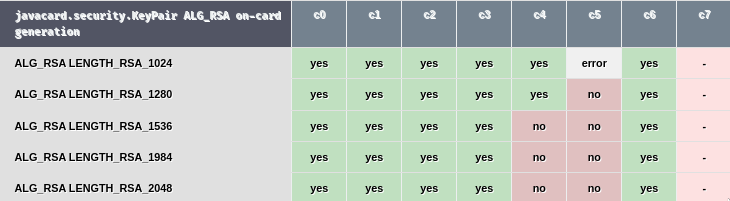
\includegraphics[width=\textwidth]{img/support-table.png}
%    \caption{Support table}
%    \label{fig:support-table}
%\end{figure}

\subsection{Similarity table}
The similarity table shows how a chosen pair of devices differ in the performance of selected groups of algorithms. High performance similarity may mean that the pair of devices have a very similar if not identical underlying hardware.

To compute pair similarity, firstly the groups of algorithms need to be selected. Then for each profile, the algorithm operation times have to be normalized, which means they will be scaled to range from 0 to 1 depending on the maximum value across all operation times for a particular algorithm. Then we can compute similarity for pairs of profiles, the measure used is based on the Euclidean distance formula.

\begin{align*}
    d(x, y) = \sqrt{\sum_{i=1}^{n}(x - y)^{2}} 
\end{align*}

Where $x$ and $y$ are normalized operation times for one algorithm supported by both devices, and $n$ is the number of these algorithms. The similarity value is finally computed as $abs(d(x, y) - 1)$, which results in a percentage in the range of 0 to 100.

%\begin{figure}[H]
%    \centering
%    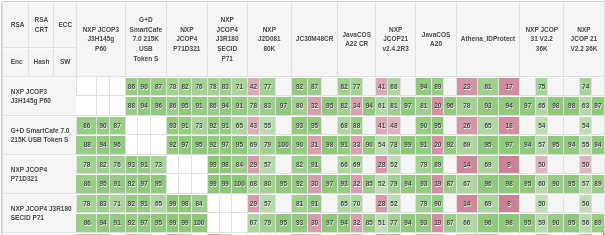
\includegraphics[width=\textwidth]{img/similarity-table.png}
%    \caption{Similarity table}
%    \label{fig:similarity-table}
%\end{figure}

\subsection{Algorithm execution time}
The algorithm execution page presents an alternative to searching in the corresponding raw CSV file representing the Performance device profiles which are mentioned in  \myref{Section}{sec:device-profiles}. 

Firstly, basic information about the device is displayed. Then several tables containing test measurements representing various algorithms with possibly differing configurations are shown. Each table represents a particular category of an algorithm. The table rows generally contain parameters of the algorithm, configuration, operation times, and information about the number of successful or unsuccessful iterations.

%\begin{figure}[H]
%    \centering
%    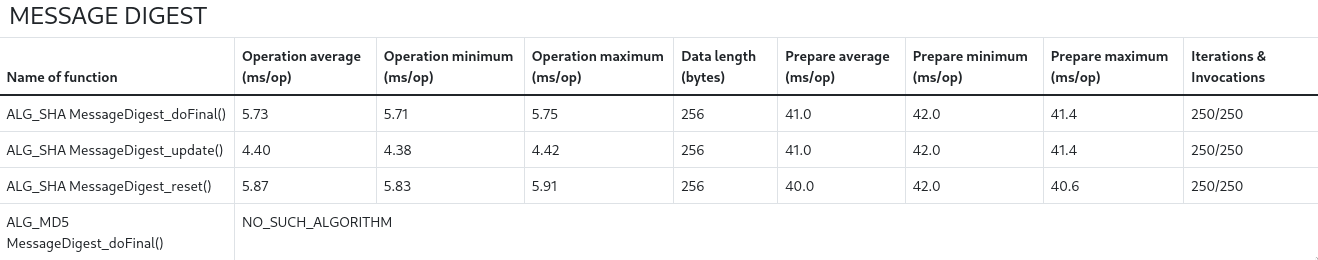
\includegraphics[width=\textwidth]{img/NXP JCOP4 P71D321 execution-time table.png}
%    \caption{Algorithm execution timetable of NXP JCOP4 P71D321}
%    \label{fig:execution-time-table}
%\end{figure}

\subsection{Radar graphs}
Radar graphs visualize the device's performance compared to all other tested cards. They can also be used for similarity comparison between two or more devices.

Likewise, as in the case of the similarity table, all algorithm operation times from a selected group need to be normalized. After the normalization, the resulting data is transformed into a JavaScript object compatible with the implementation of Radar chart visualization. Technical details of the tools used are mentioned in \myref{Section}{sec:tools}. The normalized values correspond to percentages, where the closer to 100 percent, the better the device performs compared to other devices. The algorithm identifier with an actual operation time value is shown by hovering over the edge, which is necessary in case there are too many plot axes and their captions overlap each other.

\subsection{Heatmap}
Heatmaps can be used in the analysis of generated RSA key pairs. These heatmaps visualize the distribution of most significant bytes (MSB) of RSA private primes $p$ and $q$ and their marginal histograms. The whole chart also contains a separate sub-chart with MSB histograms of these primes $p$ and $q$ and also a histogram of public moduli $n = p \cdot q$. The heatmap for the TPMs may look very sparse, but that entirely depends on the number of generated key pairs.

The motivation behind this chart comes from the research on RSA keys by Švenda et al. \cite{svenda-1mrsa_usenix2016}. They analyzed millions of key pairs generated by almost four dozen software libraries and smart cards. Their analysis revealed, among other things, that depending on the design and implementation of key generation, the origin of the key may be identified just from a public modulus $n$. That is why it may be interesting to analyze the charts that depict primes and moduli distributions for key pairs generated by the TPM devices.

The heatmap chart design is inspired by Nemec \cite{Nemec2016thesis}, but his R script for the generation of the heatmaps could not be easily reused in Python with the TPM datasets, so the plot generation had to be created in Python from the scratch.

\subsection{Comparative table}
The comparative table is used for a simple comparison between devices. When generated, the tool creates a page with several tables. Each table represents a category of algorithms whereas each column represents one algorithm from this category. The possible categories can be, for example, asymmetric algorithms, symmetric algorithms, and select frequently used algorithms.

The tables themselves allow for simple sorting according to the column values just by clicking on the selected column according to which rows will be sorted.

%\begin{figure}[H]
%    \centering
%    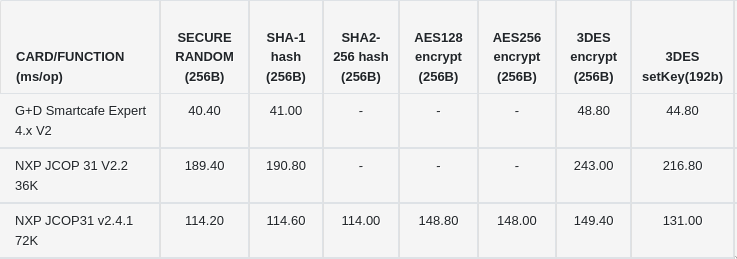
\includegraphics[width=\textwidth]{img/comparative-table.png}
%    \caption{Comparative table}
%    \label{fig:comparative-table}
%\end{figure}

\subsection{Scalability graphs}
Scalability graphs illustrate the device's performance for a specific algorithm depending on input data length. This visualization thus requires variable-length performance results, which are only collected for JavaCards.

One graph is generated for each method that was successfully measured. By hovering over the point in the graph the operation time range of the measurement along with the average operation time are shown.

%\begin{figure}[H]
%    \centering  
%    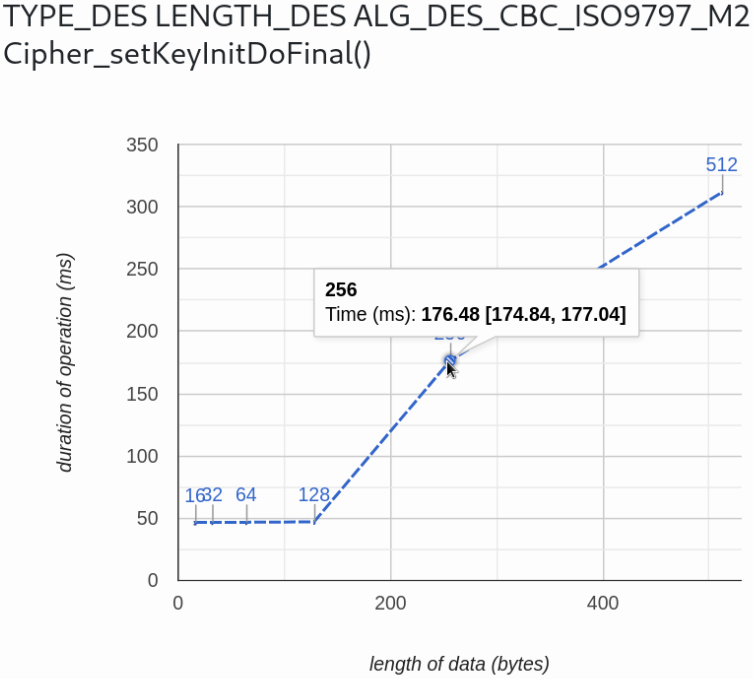
\includegraphics[width=\textwidth-3.5cm]{img/NXP_JCOP_J3D081_v2.4.2R2 scalability graph.png}
%    \caption{
%    Scalability chart of NXP JCOP J3D081 v2.4.2R2 showing performance of DES algorithm in CBC mode, for data lengths We can observe 16, 32, 64, 128 bits the performance seems to be constant, following 256, 512 bits an almost linear increase.
%    }
%    \label{fig:scalability-chart}
%\end{figure}




\section{Tools}\label{sec:tools}
The \texttt{AlgTest process} tool incorporates various instruments to produce desired outputs. As the tool itself is written in Python it is able to utilize various packages from \texttt{PyPI}\footnote{\url{https://pypi.org/}} to aid future extensions.

\begin{itemize}
    \item For creation and manipulation of HTML documents a Python library called \texttt{dominate}\footnote{\url{https://pypi.org/project/dominate/}} is used. Its usage is relatively straightforward, and the code you write is in pure python instead of using additional templating language as in popular web frameworks.
    \item The styling is taken care of by a CSS framework called \texttt{bootstrap}\footnote{\url{https://getbootstrap.com/}} which allows for designing responsive web pages using premade CSS classes and Javascript. The framework itself is extensively used and regularly updated with new versions.
    \item \texttt{Google Charts API}\footnote{\url{https://developers.google.com/chart}}  is utilized for Scalability graph visualisation.
    \item \texttt{D3.js library}\footnote{\url{https://d3js.org/}}  is used for visualisation of Radar graphs.
\end{itemize}


  
  \bookmarksetup{startatroot}

  \chapter{Conclusion}


  %% \appendix
\renewcommand{\thechapter}{A}
\chapter{Usage of AlgTest pyProcess}

\definecolor{codegreen}{rgb}{0,0.6,0}
\definecolor{codegray}{rgb}{0.5,0.5,0.5}
\definecolor{codepurple}{rgb}{0.58,0,0.82}
\definecolor{backcolour}{rgb}{0.95,0.95,0.92}

\lstdefinestyle{mystyle}{
    backgroundcolor=\color{white},   
    commentstyle=\color{codegreen},
    keywordstyle=\color{magenta},
    numberstyle=\tiny\color{codegray},
    stringstyle=\color{codepurple},
    basicstyle=\ttfamily\footnotesize,
    breakatwhitespace=false,         
    breaklines=true,                 
    captionpos=b,                    
    keepspaces=true,                          
    showspaces=false,                
    showstringspaces=false,
    showtabs=false,                  
    tabsize=2
}

\lstset{style=mystyle}

\section{Installation}
After cloning into repository containing \texttt{AlgTest process} tool, it is necessary to install a few dependencies. The project includes a script called \texttt{setup.py} which, when ran installs required packages. It may be convenient to create a Python virtual environment that allows us to install and manage Python project packages locally without unnecessary global installation. It is important to create and source a virtual environment before running the setup script.
\begin{lstlisting}[language=bash]
    $ python -m venv venv
    $ source venv/bin/activate
    $ python setup.py
\end{lstlisting}

\section{Folder structure}
\begin{itemize}
    \item \texttt{algtestprocess}
        \begin{itemize}
            \item \texttt{modules} -- folder containing \texttt{algtestprocess} modules.
                \begin{itemize}
                    \item \texttt{components} -- folder containing reusable code for parts of HTML documents. Each file contains classes, constants related to one component.
                    \item \texttt{pages} -- folder containing files with classes corresponding to generated HTML pages, each page has a separate file containing class which is responsible for page creation.
                    \item \texttt{parser}
                        \begin{itemize}
                            \item \texttt{javacard} -- folder containing parser implementations for JavaCard profiles
                            \item \texttt{tpm} -- folder containing parser implementations for TPM profiles
                        \end{itemize}
                    \item \texttt{config.py} -- file containing classes for choice of algorithms used in specific pages
                    \item \texttt{jcalgtest.py} -- file containing classes for storage of Java Card profiles
                    \item \texttt{tpmalgtest.py} -- file containing classes for storage of TPM profiles
                \end{itemize}
        \end{itemize}
    \item \texttt{setup.py} -- script for installation of dependencies and download of results from their official GitHub repository\footnote{\url{https://github.com/crocs-muni/jcalgtest_results}}
    \item \texttt{process.py} -- main entrypoint for generation of outputs, its usage is described in following section
\end{itemize}

\section{Usage}
The script process.py provides a CLI in the following way:

\begin{itemize}
    \item Set of operations from \texttt{process, all, execution-time, comparative, radar, scalability, similarity, support}. We can select multiple operations; however, \texttt{process} operation needs to be run at least once so that some issues with CSV files are fixed, and JSON outputs are generated for the following operations which use them. In the subsequent runs the \texttt{process} argument is not necessary.
    \item \texttt{-i/-{}-results-dir} A directory with measurement results.
    \item \texttt{-o/-{}-output-dir} Output directory to which the HTML outputs are stored.
\end{itemize}

\begin{lstlisting}[language=bash]
    $ python process.py process all --results-dir ./jcalgtest_results/ --output-dir ./jcalgtest_results/javacard/web
    $ python process.py radar scalability -i ./jcalgtest_results/ -o ./jcalgtest_results/javacard/web
\end{lstlisting}

\renewcommand{\thechapter}{B}
\chapter{Diagrams and Visualizations}\label{appendix:diagrams-visualizations}

\begin{figure}[H]
    \centering
    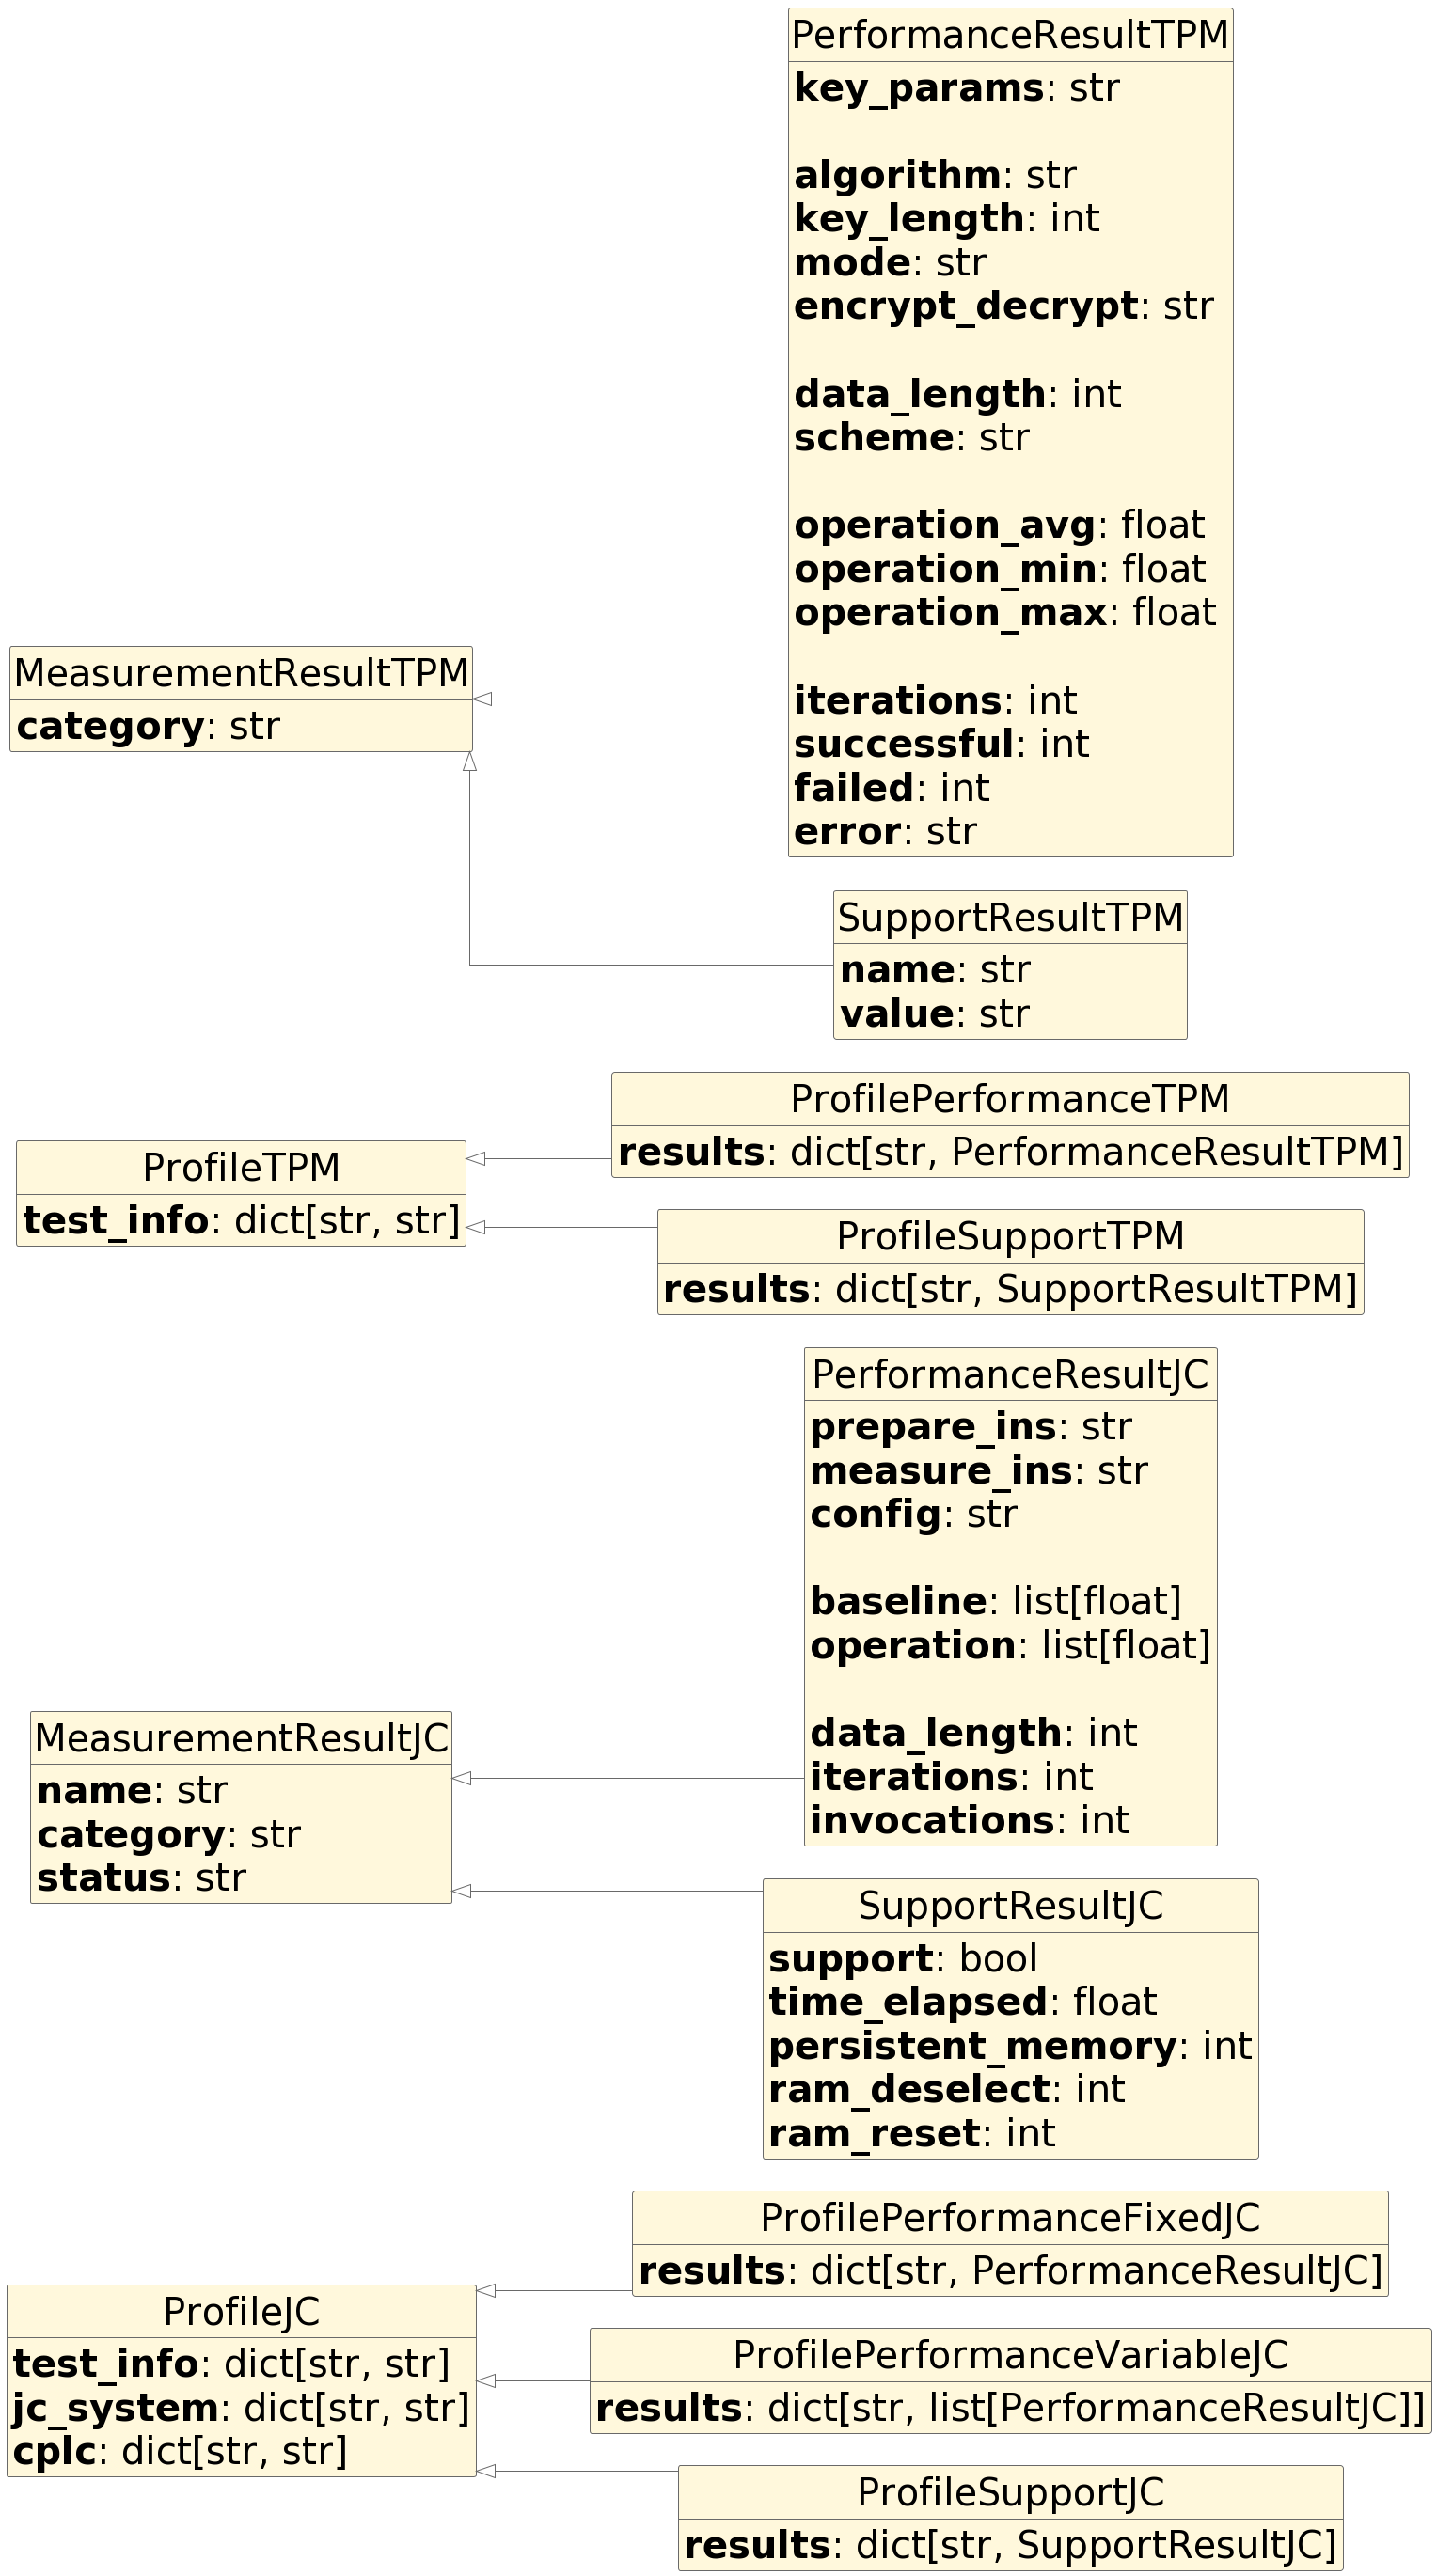
\includegraphics[width=\textwidth,height=\textheight-4.5cm, keepaspectratio]{img/diagrams/object_diagram.png}
    \caption{Diagram of Device profiles}
    \label{fig:dev-profiles-diagram}
\end{figure}

\begin{landscape}
    \begin{figure}[!t]
        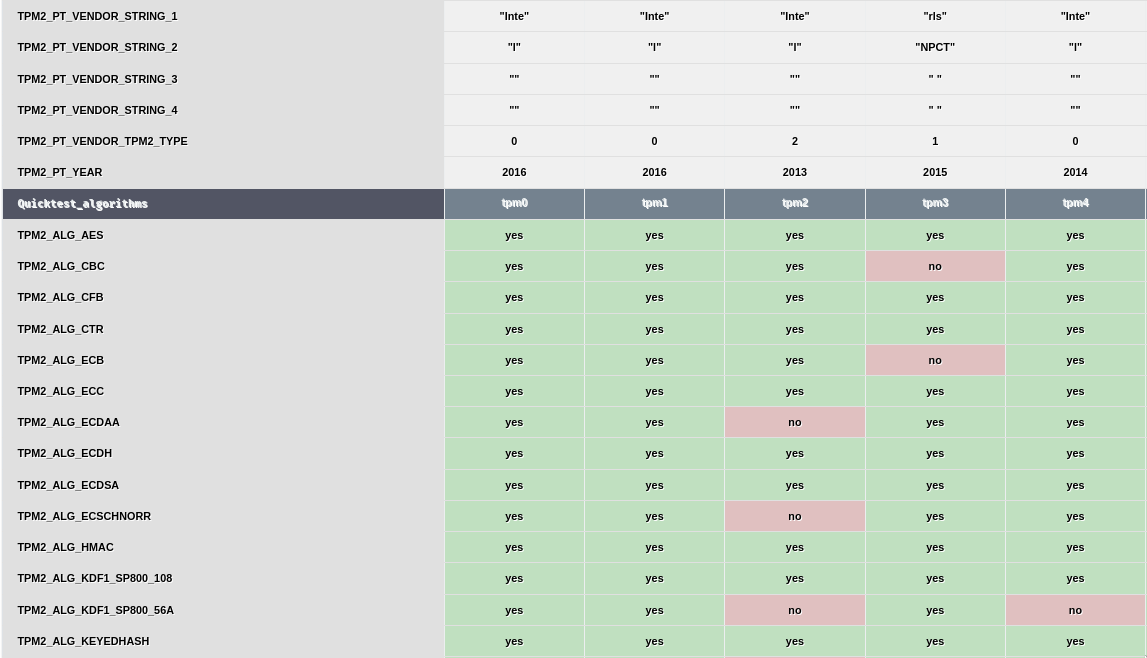
\includegraphics[width=\linewidth, height=\textwidth]{img/visualizations/tpm-support-data.png}
        \caption{An example of a part of Support table visualization for the TPMs}
    \end{figure}
\end{landscape}

\begin{landscape}
    \begin{figure}[!t]
        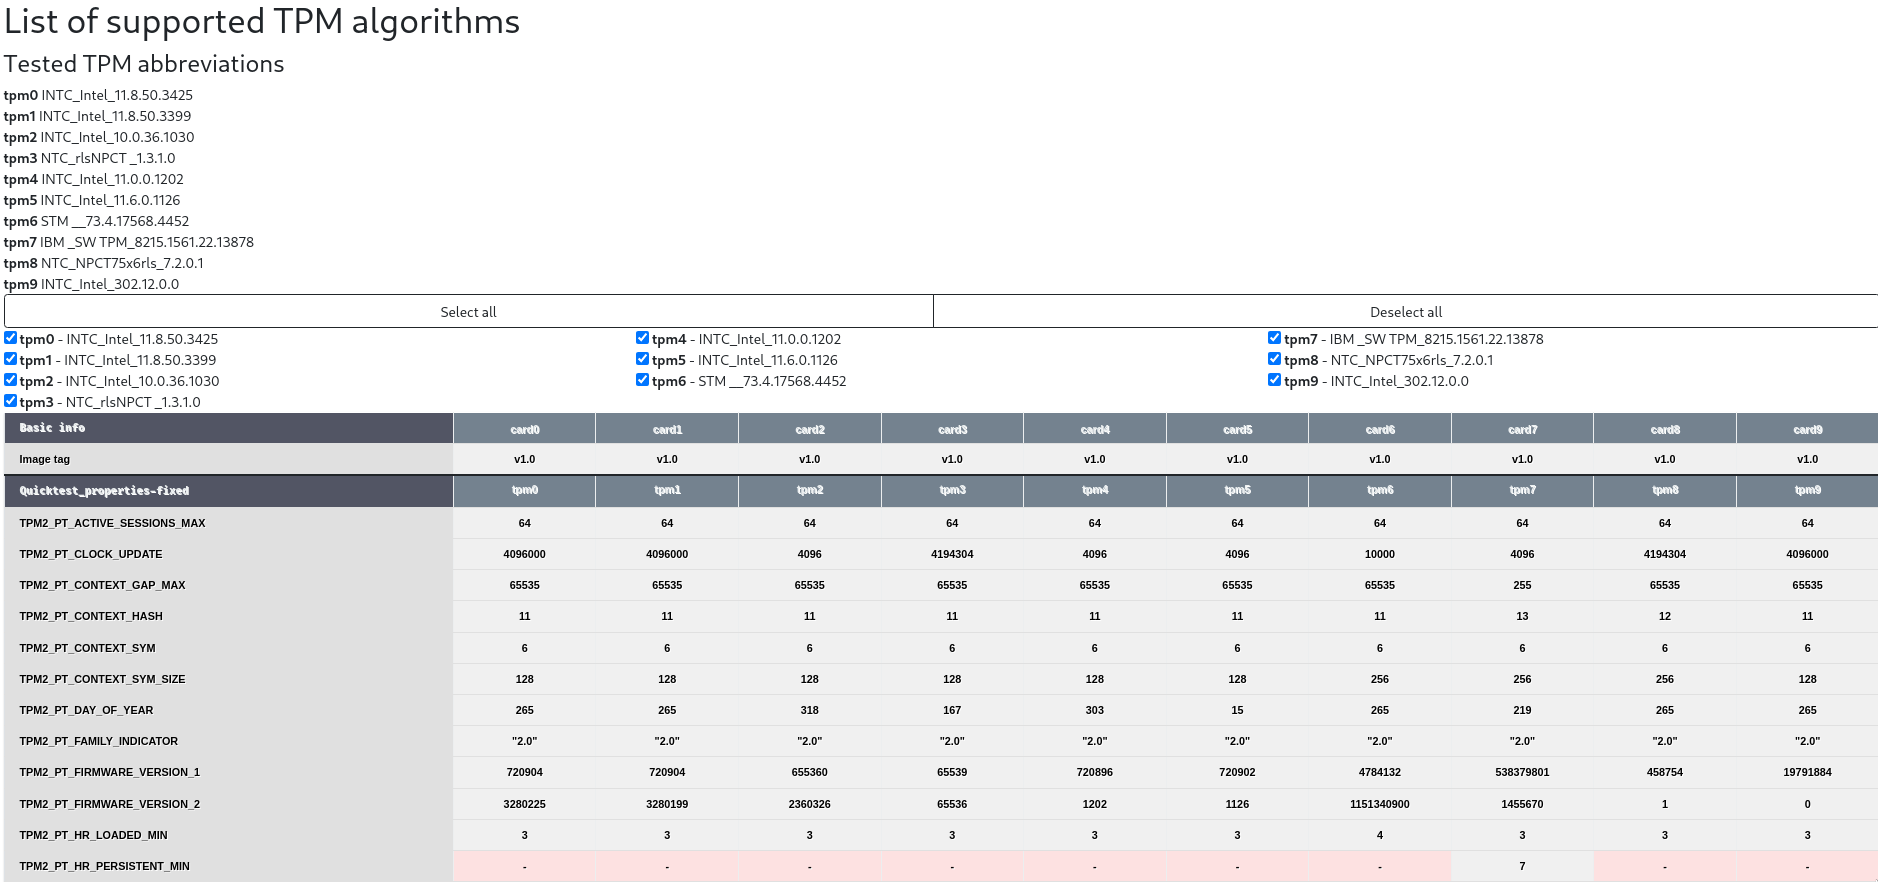
\includegraphics[width=\linewidth, height=\textwidth]{img/visualizations/tpm-support-utility.png}
        \caption{Support tables also contain checkbox utility for filtering the devices}
    \end{figure}
\end{landscape}

\begin{landscape}
    \begin{figure}[!t]
        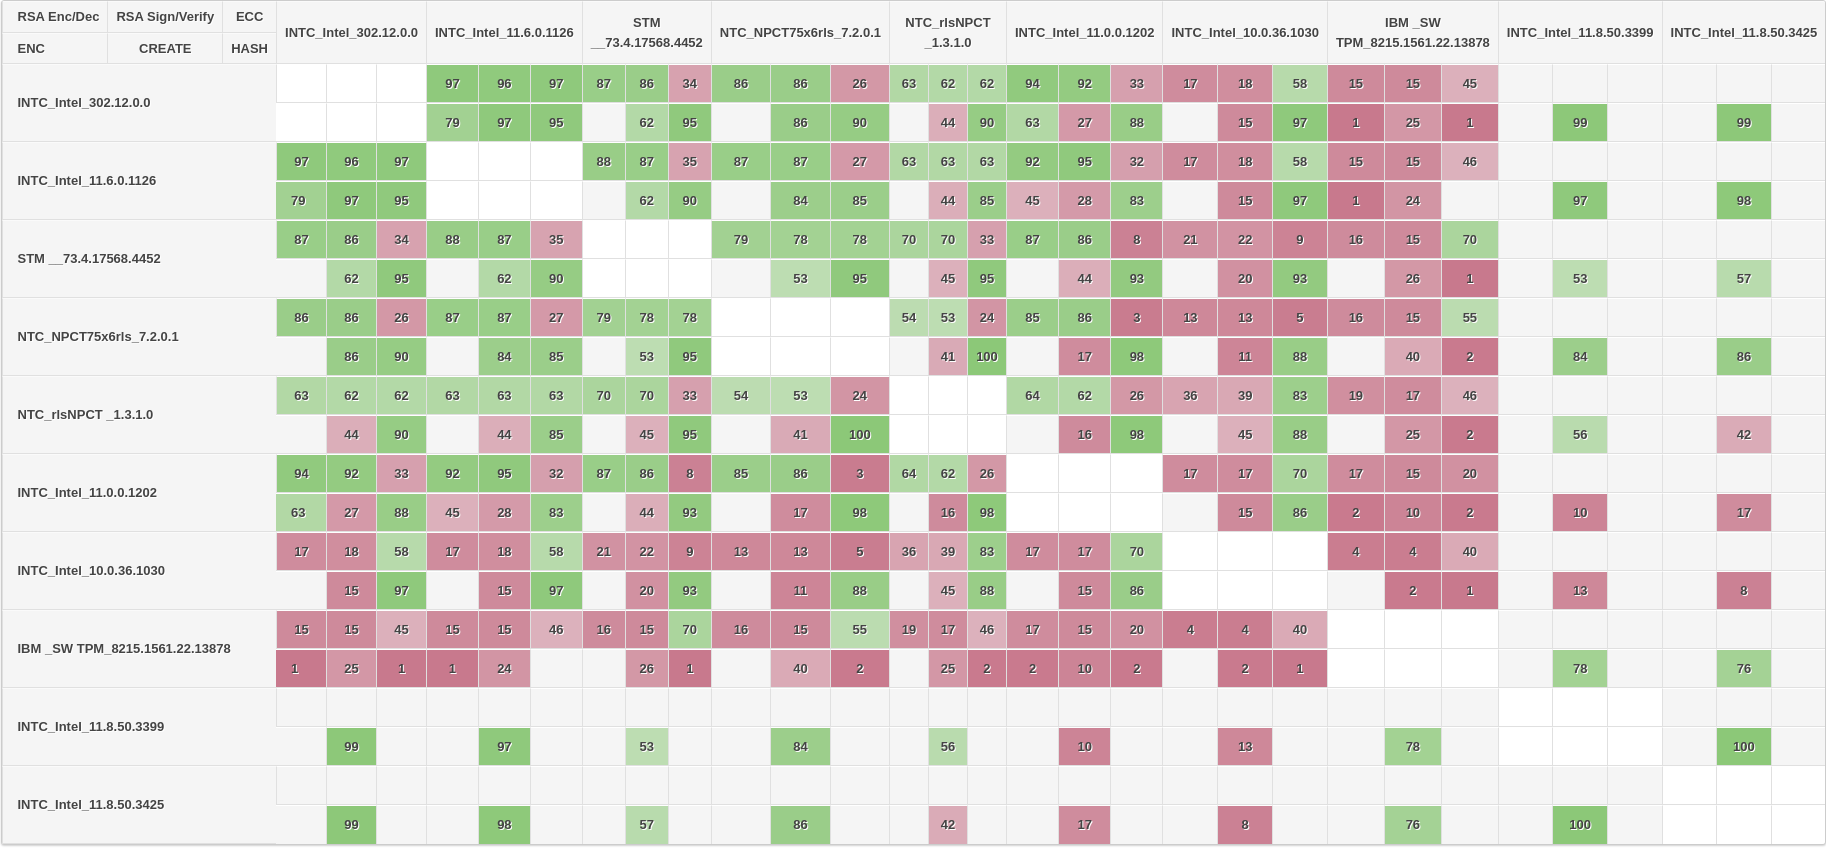
\includegraphics[width=\linewidth, height=\textwidth]{img/visualizations/tpm-similarity.png}
        \caption{Similarity table for TPMs}
    \end{figure}
\end{landscape}

\begin{landscape}
\begin{figure}[!t]
    \centering
    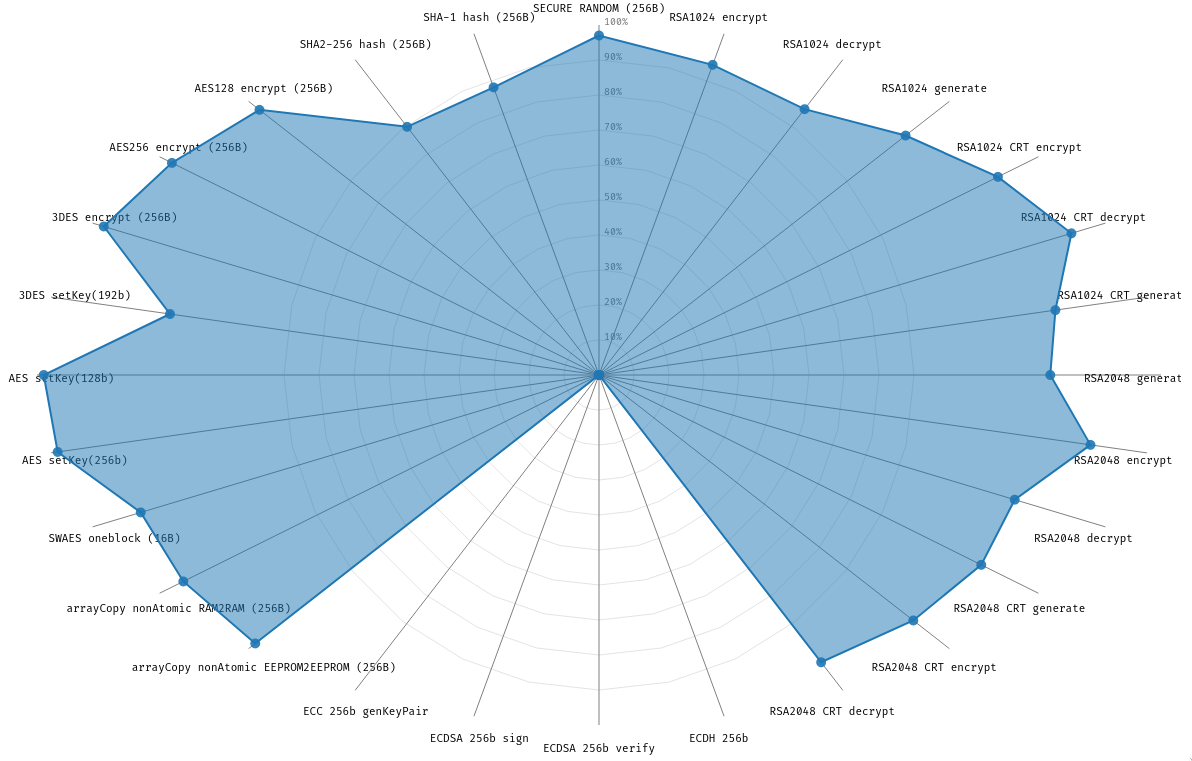
\includegraphics[width=\linewidth]{img/visualizations/JC30M48CR radar graph.png}
    \caption{
    The radar graph of the JC30M48CR smart card. Its performance can be considered excellent, apart from no evident support for algorithms involving Elliptic Curve Cryptography signified by a cut-out at the bottom of the graph.
    }
\end{figure}
\end{landscape}

\begin{landscape}
\begin{figure}[!t]
    \centering
    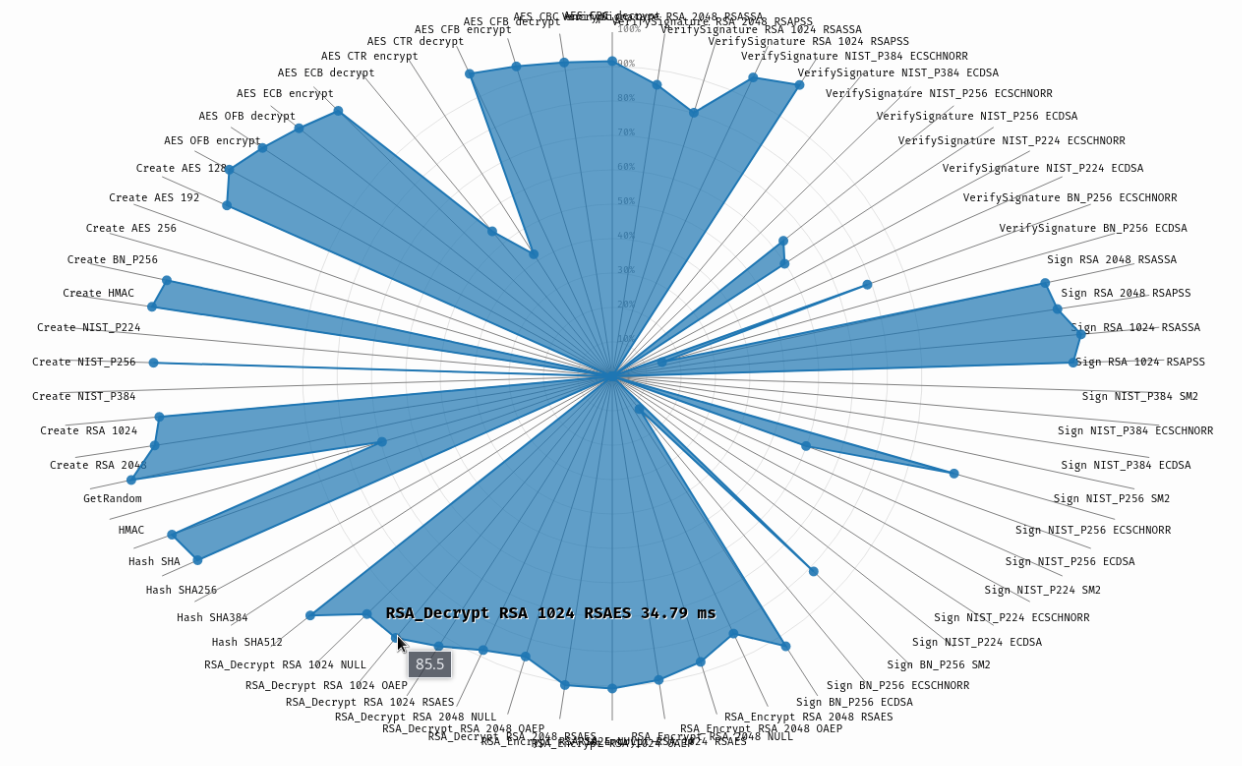
\includegraphics[width=\linewidth]{img/visualizations/INTC_Intel_302.12.0.0 radar graph.png}
    \caption{
    The radar graph of the INTC Intel 302.12.0.0 TPM.
    }
\end{figure}
\end{landscape}
\begin{figure}[H]
    \centering
    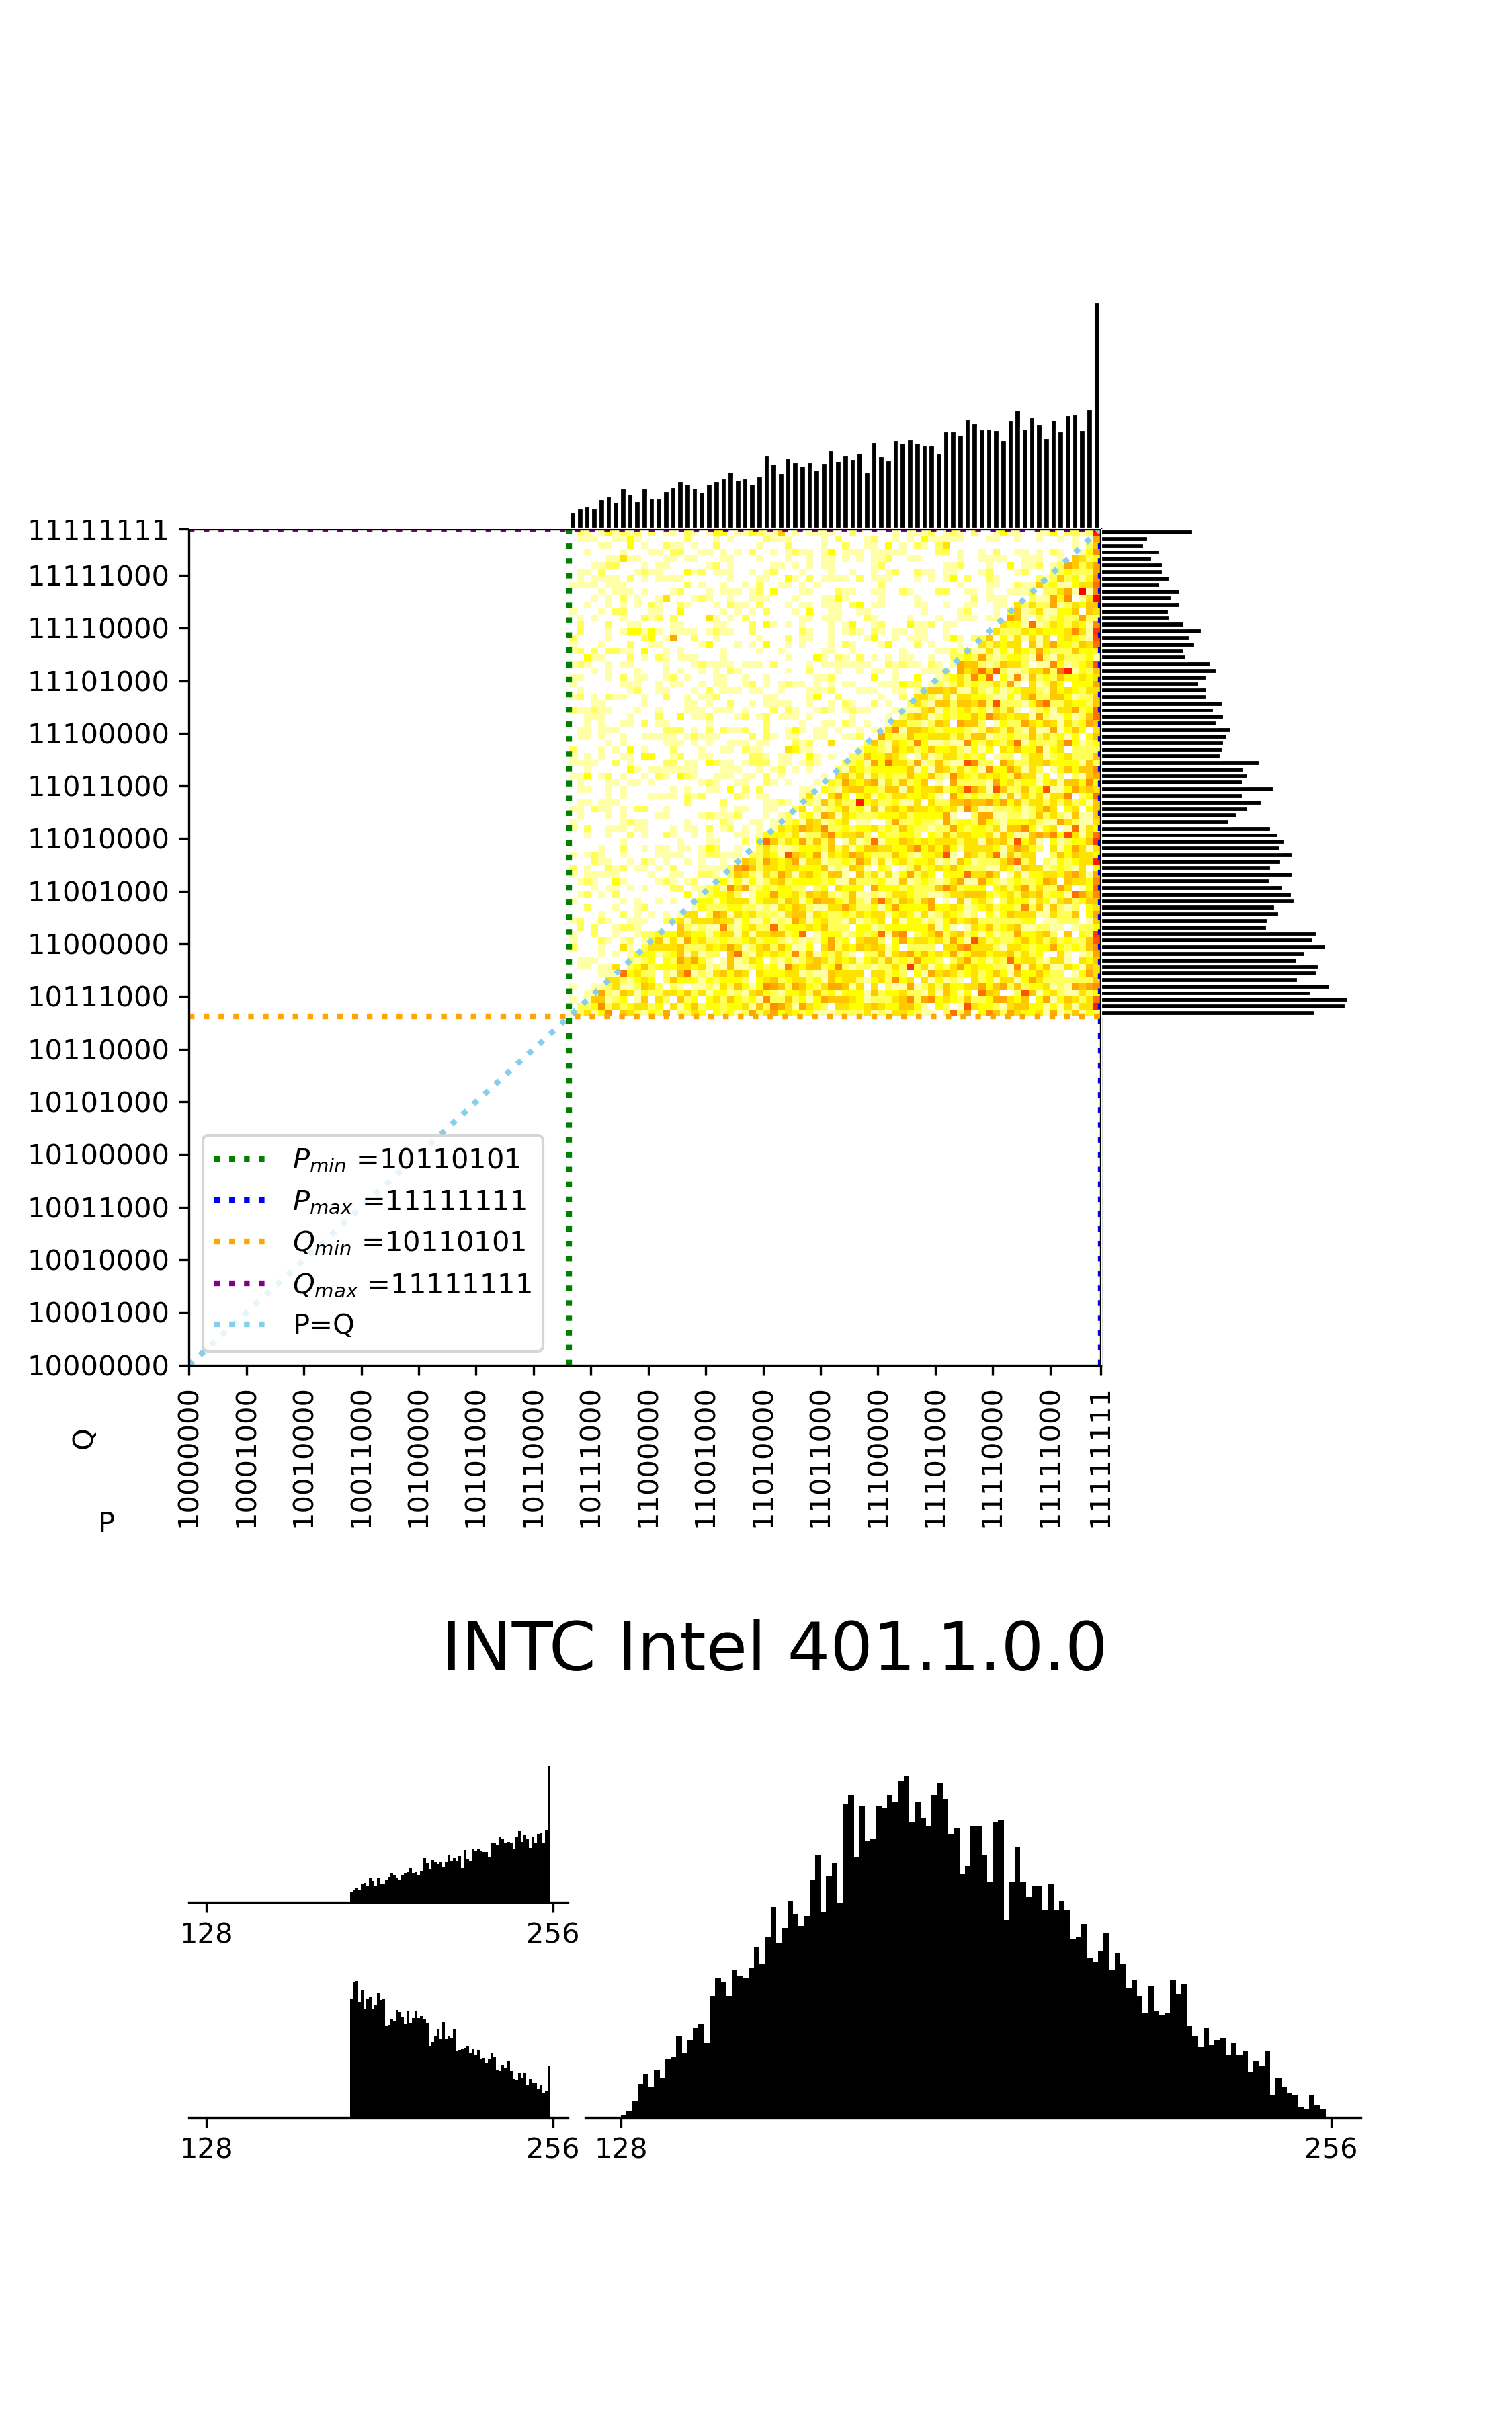
\includegraphics[width=\textwidth,height=\textheight-1.5cm, keepaspectratio]{img/visualizations/rsa.png}
    \caption{TPM chart showing the heatmap and several histograms of most significant bytes of gathered 1024 bit RSA keys.}
    \label{fig:dev-profiles-diagram}
\end{figure}





\renewcommand{\thechapter}{C}
\chapter{Data Attachments}
  \backmatter
  \printindex
  \begingroup
  \sloppy

  \printbibliography
\endgroup


\end{document}

